\chapter{From First Commission to Brokerage Ownership}

This chapter is built from the interview's spoken arithmetic rather than from displayed board work. Even so, the lecture has a clear quantitative spine. We begin with a money shock, then move through the accumulation of a real-estate skill stack, the threshold logic of brokerage, the economics of partnership, and finally the arithmetic of a large wholesale transaction, a large capital loss, and a long-range entrepreneurial goal. The important thing is to keep the order of revelation intact. The speaker does not start with a theory. He starts by seeing a check.

\section{Opening Shock and Formal Reset}

We begin where the lecture begins: with a discontinuity. A young prospective agent sits in a brokerage office and watches a local operator receive a \(\$200{,}000\) check. A few sentences later the scene collapses into ordinary wage life: pizza delivery, mopping floors, and then a first closing worth roughly \(\$6{,}000\) to \(\$7{,}000\). The interview wants us to feel that gap before it explains it.

\paragraph{Anecdote.}
The first image is not educational prestige or firm ownership. It is a single payment. Then, just as quickly, the speaker places himself back inside low-wage routine. The cold open therefore gives us two scales of economic life at once.

\paragraph{Claim.}
The lecture's opening claim is that entrepreneurial opportunity first becomes believable through scale perception. One does not slowly reason one's way from a \(\$600\) paycheck into the world of six-figure closings. One first sees that the larger world exists.

\paragraph{Mechanism.}
What the cold open does narratively, the formal interview then does structurally. The host resets the scene, introduces Matt Teifke and Teifke Real Estate, and names the present goal: to build the most entrepreneurial brokerage on the planet. That reset matters. The opening gave the payoff first; the interview now promises to explain how one gets there.

\section{Biography as Accumulation, Not Sudden Genius}

Once the present ambition has been named, the lecture steps backward and begins to build the ladder. We are given childhood, family influence, early licensing, college, graduate study, appraisal work, apartment experience, third-party management, company sale, and then the later partnership that produces the current brokerage.

\paragraph{Anecdote.}
The sequence is concrete. The speaker grows up with a single mother who makes real estate seem possible, gets licensed at \(17\), studies real estate finance, works across multiple parts of the business, starts a company with his wife, scales it to hundreds of managed doors, sells it, and then builds again with a childhood friend.

\paragraph{Claim.}
Ownership is presented here as accumulation. The lecture is careful not to treat success as one lucky deal or one magic credential. Instead, it treats entrepreneurship as layered contact with the same field from several operational viewpoints.

\paragraph{Mechanism.}
The scale markers are worth preserving because they show the shape of the climb:
\begin{equation}
17 \text{ years old at licensing}, \qquad
700 \text{ doors managed}, \qquad
130 \text{ properties later held}.
\end{equation}
These are not decorative numbers. They tell us that the speaker keeps moving from access to responsibility: first learning how the business works, then learning how it is valued, then learning how it is operated, and only then trying to own a larger share of it.

\section{College, Credentials, and Network Value}

At this point the biography naturally raises a conventional question: if college and graduate study are in the story, how much of the outcome depends on formal education?

\subsection{Question \& Answer}

\paragraph{Question.}
Is college necessary for success in real estate and in business more generally? And if it is not strictly necessary, what was its real value?

\paragraph{Answer.}
The answer is neither a defense of credentialism nor a ritual rejection of school. The speaker says no, college is not necessary in any absolute sense. But he immediately reframes the issue. Education is an environment whose value depends on what one makes of it. A room full of people interested in business already contains future collaborators; the waste lies in treating such a room as a place one merely enters and leaves.

\paragraph{Mechanism.}
The lecture therefore gives education two distinct entrepreneurial functions:
\begin{itemize}
\item It can satisfy formal requirements later in the path.
\item It can provide access to peers whose ambition is available but not yet organized.
\end{itemize}
The point is subtle and worth preserving. The interview does not say, ``credentials do not matter.'' It says that the value of an institution depends on whether we turn proximity into cooperation.

\section{First Entry, First Deal, and the First Real Money}

Having answered the question about education, the host deliberately rewinds the lecture. We are asked to return to the beginning and explain how the speaker first entered real estate and what the first real money looked like.

\subsection{Question \& Answer}

\paragraph{Question.}
How did the first involvement in real estate actually happen, and what was the first deal or the first real income event?

\paragraph{Answer.}
The first surprise is structural. The novice agent thinks he is interviewing for permission to enter the business, but in fact brokerages want new agents. The second surprise is dramatic. During one of those meetings a local broker receives a \(\$200{,}000\) check and turns it into a form of mentorship: you can get there too.

\paragraph{Anecdote.}
The speaker then takes the opportunity but keeps delivering pizza, because one still needs immediate cash flow. The first real-estate call arrives while he is mopping the floor. He drops the mop, takes the call, closes the deal, and receives a commission so much larger than his ordinary paycheck that the business becomes irreversible in his imagination.

\paragraph{Mechanism.}
If we write the first closing as \(F\) and the prior paycheck scale as \(W\), the opening shock becomes measurable:
\begin{align}
F &\approx 6{,}000 \text{ to } 7{,}000,\\
W &\approx 600,\\
R_{\mathrm{shock}} &= \frac{F}{W} \approx 10 \text{ to } 11.7.
\end{align}
Even against a larger full-time paycheck scale of roughly \(\$1{,}500\) to \(\$2{,}000\), we still do not get a small increment. We get a multiple:
\begin{equation}
\frac{6{,}000}{2{,}000}=3,
\qquad
\frac{7{,}000}{1{,}500}\approx 4.7.
\end{equation}
This is the first genuine piece of arithmetic in the lecture. A one-time commission does not merely add cash. It rescales the opportunity set.

\section{From Agent to Broker: Threshold Logic and Split Economics}

Once the first-deal story is fully told, the host asks the next natural question. If a first commission explains why one becomes serious, how does one move from being an agent inside another person's structure to becoming the broker who runs the platform?

\subsection{Question \& Answer}

\paragraph{Question.}
What changes when an agent becomes a broker?

\paragraph{Answer.}
The answer has two layers. First, there is threshold logic: years of experience, transactions, points, and required coursework. Second, there is a change in the nature of responsibility. The broker becomes the party under whom agents work, the party who trains, supports, and remains legally and operationally exposed.

\begin{definition}[Broker in the sense of the interview]
A broker is the supervisory licensed party under whom agents operate. In the lecture's language, the broker is responsible, on the hook, and charged with training and supporting the platform.
\end{definition}

The spoken threshold structure can be written compactly as
\begin{equation}
Y_{\mathrm{req}}^{\mathrm{old}} = 2 \text{ years},
\qquad
Y_{\mathrm{req}}^{\mathrm{new}} = 4 \text{ years},
\qquad
P_{\mathrm{req}} \approx 900.
\end{equation}
The speaker also says that college and graduate study satisfied the credit-hour side of the requirement, so the licensing threshold is a conjunction of time, transaction logic, and coursework rather than a single hurdle.

\begin{table}[h]
\centering
\begin{tabular}{p{0.30\linewidth}p{0.56\linewidth}}
Requirement & Interview description \\
Experience & Earlier rule of two years, later changed to four years \\
Transaction logic & Point system, stated at about \(900\) points \\
Coursework & Required credit hours; speaker says prior degrees satisfied them \\
Institutional change & Broker trains, supports, supervises, and remains on the hook \\
\end{tabular}
\caption{Transcript-based summary of the move from agent to broker.}
\end{table}

Once the threshold logic is stated, the interview turns immediately to platform economics. If \(C\) denotes gross commission, then the current and earlier split structures are
\begin{align}
C_{\mathrm{agent}} &= 0.9\,C,
&
C_{\mathrm{brokerage}} &= 0.1\,C,
\\
C_{\mathrm{agent}}^{\mathrm{old}} &= 0.5\,C,
&
C_{\mathrm{brokerage}}^{\mathrm{old}} &= 0.5\,C.
\end{align}

\paragraph{Worked example.}
Take a gross commission of \(C=10{,}000\). Then
\begin{equation}
C_{\mathrm{agent}}^{90/10}=9{,}000,
\qquad
C_{\mathrm{agent}}^{50/50}=5{,}000.
\end{equation}
So the current model gives the agent
\begin{equation}
\frac{0.9C}{0.5C}=1.8
\end{equation}
times the gross share that the earlier \(50\text{--}50\) arrangement would have given. This is why the split belongs in the chapter. Brokerage is not only a licensing status; it is a platform design.

\begin{remark}
The licensing rules are reported conversationally, not as statute. We should therefore preserve them as approximate spoken thresholds rather than quote them as legal code.
\end{remark}

\section{Leadership Burden and Partnership Design}

Once the structure of brokerage is clear, the host asks what it feels like to run such a platform. The lecture now shifts from thresholds to strain.

\paragraph{Anecdote.}
The speaker names the familiar forms of operating disorder: deals fall apart, lawsuits appear, complaints accumulate, and yet leadership still has to look like leadership. One may be carrying private difficulty while still being responsible for the morale and momentum of others.

\paragraph{Claim.}
Ownership is therefore not reducible to upside. The lecture insists that it is a burden-bearing role. That is exactly why the conversation widens into partnership. If the burden is real, then the right counterpart becomes a serious economic variable.

\subsection{Question \& Answer}

\paragraph{Question.}
What should one look for in a business partner?

\paragraph{Answer.}
The answer begins pessimistically: very few partnerships work. The lecture does not ask us to romanticize partnership. It asks us to explain why this one survived.

\paragraph{Mechanism.}
The speaker's answer is evidence-based. He names a long preexisting relationship, a period of distrust because of the partner's earlier life, repeated demonstrations of work ethic, and finally a role division that became stable because it matched actual strengths rather than slogans.

The sequence of tests is important:
\begin{itemize}
\item The relationship is not new; it is built on long familiarity.
\item The partner's early trajectory gave reasons for caution rather than easy trust.
\item When given work, he repeatedly overperformed.
\item Sobriety and discipline were not asserted once; they were demonstrated over time.
\item Complementarity was established operationally, not rhetorically.
\end{itemize}

\begin{table}[h]
\centering
\begin{tabular}{p{0.42\linewidth}p{0.42\linewidth}}
Implementer side & Visionary side \\
Counts money and guards profitability & Networks and builds relationships \\
Handles hiring and firing & Generates new ideas \\
Runs operations and execution & Extends the firm's reach \\
Stabilizes the platform & Expands the platform \\
\end{tabular}
\caption{Transcript-based division of labor in the partnership.}
\end{table}

The interview names this pairing through the language of Traction: the implementer and the visionary. What matters for the notes is the underlying point. A partnership works when imagination and execution are both present and are not confused with one another.

\section{Capital Events: Wholesaling, Drawdown, and Long-Horizon Judgment}

Only after the lecture has passed through entry, licensing, leadership, and partnership does it reach the largest financial claims. This order is important. The big deal comes late because the lecture wants us to understand the machinery that makes such a deal intelligible.

\subsection{Question \& Answer}

\paragraph{Question.}
What was the biggest deal, and how did it work?

\paragraph{Answer.}
The answer is a wholesaling story. A property is put under contract at one price, control over that contract is secured by earnest and option money, a higher-paying buyer is found, and the spread between the two prices becomes the core economic event.

\begin{definition}[Wholesale spread]
In the narrow sense used in this interview, we secure control over a property contract at price \(V_{\mathrm{contract}}\) and later monetize that control at an effective exit value \(V_{\mathrm{exit}}\). The gross spread is
\begin{equation}
S = V_{\mathrm{exit}} - V_{\mathrm{contract}}.
\end{equation}
\end{definition}

The spoken figures are approximately
\begin{equation}
V_{\mathrm{contract}} \approx 2.0\,\mathrm{M},
\qquad
V_{\mathrm{exit}} \approx 2.7\,\mathrm{M},
\qquad
E_{\mathrm{earnest+option}} \approx 20{,}000.
\end{equation}

\begin{figure}[h]
\centering
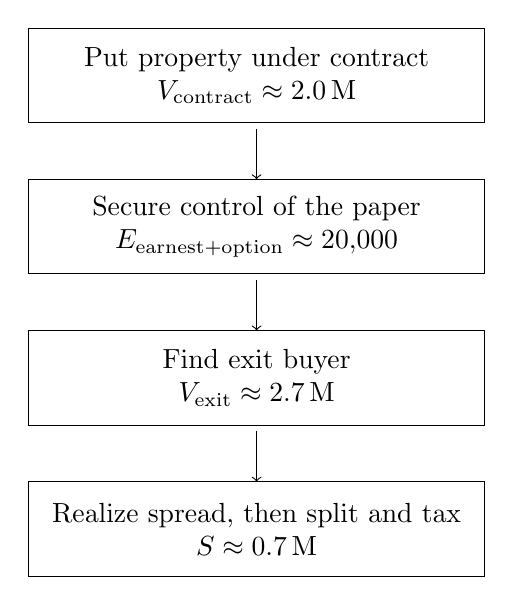
\begin{tikzpicture}[x=1cm,y=1cm]
\draw (0,0) rectangle (5.8,1.2);
\node[align=center] at (2.9,0.6)
{Put property under contract\\
\(V_{\mathrm{contract}} \approx 2.0\,\mathrm{M}\)};

\draw[->] (2.9,-0.08) -- (2.9,-0.72);

\draw (0,-1.92) rectangle (5.8,-0.72);
\node[align=center] at (2.9,-1.32)
{Secure control of the paper\\
\(E_{\mathrm{earnest+option}} \approx 20{,}000\)};

\draw[->] (2.9,-2.00) -- (2.9,-2.64);

\draw (0,-3.84) rectangle (5.8,-2.64);
\node[align=center] at (2.9,-3.24)
{Find exit buyer\\
\(V_{\mathrm{exit}} \approx 2.7\,\mathrm{M}\)};

\draw[->] (2.9,-3.92) -- (2.9,-4.56);

\draw (0,-5.76) rectangle (5.8,-4.56);
\node[align=center] at (2.9,-5.16)
{Realize spread, then split and tax\\
\(S \approx 0.7\,\mathrm{M}\)};
\end{tikzpicture}
\caption{Transcript-based schematic of the wholesale transaction.}
\end{figure}

\paragraph{Worked derivation.}
The lecture's own arithmetic can be written in the order in which it is narrated:
\begin{align}
S &= V_{\mathrm{exit}} - V_{\mathrm{contract}},\\
&\approx 2.7\,\mathrm{M} - 2.0\,\mathrm{M},\\
&= 0.7\,\mathrm{M}.
\end{align}
This matches the repeated \(\$700{,}000\) scale in the interview, though the speaker also mentions \(\$780{,}000\). We should therefore preserve the number as approximate rather than over-settle it.

There is a second piece of arithmetic here, and it explains why wholesaling feels powerful. A relatively small amount of cash controls a much larger contractual position. If we define
\begin{equation}
L_{\mathrm{control}}=
\frac{V_{\mathrm{contract}}}{E_{\mathrm{earnest+option}}},
\end{equation}
then the spoken numbers give
\begin{equation}
L_{\mathrm{control}}
\approx
\frac{2{,}000{,}000}{20{,}000}
=100.
\end{equation}
This is best understood as contract-control leverage: a small committed amount secures rights over a much larger transaction path.

\begin{remark}
The interview says that control of the paper is ``actual ownership.'' We should phrase this carefully in the final notes. The economically clean point is control over the contract and therefore over the spread opportunity.
\end{remark}

The interview then performs a correction which is easy to lose if one writes too quickly. Headline gross numbers are not retained wealth. The deal still passes through a partner split, taxes, and possibly a separate commission claim whose precise relation to the spread is not fully clear in the audio.

If \(G\) denotes the gross fee headline and if the deal is shared across \(n_p=3\) partners, then the pre-tax equal split is
\begin{equation}
G_{\mathrm{per\ partner}} = \frac{G}{3}.
\end{equation}
For the two numbers spoken in the interview this becomes
\begin{equation}
\frac{700{,}000}{3}\approx 233{,}333,
\qquad
\frac{780{,}000}{3}=260{,}000.
\end{equation}
If we write the effective tax fraction abstractly as \(\tau\), then the same logic yields
\begin{equation}
G_{\mathrm{net,\ partner}} \approx (1-\tau)\frac{G}{3},
\end{equation}
before any further complications. This is enough to preserve the speaker's point: gross headlines exaggerate retained wealth.

\begin{table}[h]
\centering
\begin{tabular}{p{0.42\linewidth}p{0.40\linewidth}}
Layer & Approximate interview quantity \\
Contract price & \(\$2.0\,\mathrm{M}\) \\
Exit price & \(\$2.7\,\mathrm{M}\) \\
Spread scale & \(\$700{,}000\), with \(\$780{,}000\) also mentioned \\
Upfront control money & about \(\$20{,}000\) \\
Equal partner split & about \(\$233{,}333\) to \(\$260{,}000\) before tax \\
Additional commission & \(3\%\) mentioned, but exact placement is uncertain \\
\end{tabular}
\caption{Gross-to-net structure of the biggest deal, kept deliberately approximate.}
\end{table}

\subsection{Question \& Answer}

\paragraph{Question.}
What were the best and worst financial decisions?

\paragraph{Answer.}
The worst decision, by the speaker's own account, was cannabis stock. The best decision was partnership with Alex. The interview therefore places a speculative capital drawdown and an organizational success side by side.

\paragraph{Mechanism.}
The downside is reported in daily, not merely annual, terms:
\begin{align}
\Delta V_{\mathrm{day}} &\approx -(60\text{k to }100\text{k}),\\
R_q &\approx 67\,\mathrm{M},\\
M &\approx 40\,\mathrm{M}.
\end{align}
If we compress the speaker's valuation intuition into simple bookkeeping ratios, we obtain
\begin{equation}
\frac{M}{R_q} \approx \frac{40}{67} \approx 0.60,
\qquad
\frac{M}{4R_q} \approx \frac{40}{268} \approx 0.15.
\end{equation}
These are not valuation theorems. They are the arithmetic underneath the speaker's own claim that the business is undervalued and that the position is ``early'' rather than merely broken.

\paragraph{Claim.}
The deeper judgment of the section is more interesting than the stock itself. The lecture finally says that the best financial decision was choosing the right partner. That is a strong entrepreneurial statement: organization can dominate speculation.

\paragraph{Closing movement.}
The interview does not end on the trade. It moves through strange field stories and then asks about the next ten years. The final answer returns to clarity of goal, daily proof from agents whose lives have changed, and the sustaining force of a defined direction. In that sense the closing resolves the opening. Money remains central, but the mature form of the lecture is no longer just a large check. It is a structure one is trying to build.

\section{Summary}

The lecture begins by letting us see scale before it lets us understand process. We watch a \(\$200{,}000\) check appear, then we follow the speaker backward into the mechanisms that make such an event intelligible: licensing, education, appraisal, management, brokerage, partnership, wholesaling, and capital risk.

The durable lessons can be stated briefly.

\begin{itemize}
\item Entrepreneurial opportunity often becomes real through a discontinuity in scale.
\item Real-estate ownership is built by stacking several operational viewpoints rather than by relying on one credential.
\item Education matters most when it is converted into relationships and coordinated effort.
\item Brokerage introduces threshold logic and supervisory responsibility.
\item Split structure is not a minor detail; it defines the economics of the platform.
\item Partnership must be tested by evidence, discipline, and complementary roles.
\item Large deals are not merely large numbers; they are spreads, control rights, splits, and taxes.
\item Long-run judgment is finally social as much as financial: the right partner may be the best decision in the whole interview.
\end{itemize}

So the chapter closes where the lecture itself closes. We do not merely chase larger checks. We move from isolated income events toward repeatable structures of control, support, risk-bearing, and clear entrepreneurial purpose.